\chapter{Annex}\label{ch:annex}

\section{Rule extraction algorithms descriptions}\label{sec:annex-rule-extraction}
\hyperref[alg:annex-oneclasssvmXAI]{Algorithm} \ref{alg:annex-oneclasssvmXAI} contains the proposal for rule extraction for an OCSVM model that may be applied over a data set with either categorical or numerical variables (or both).
\textit{ocsvm\textunderscore rule\textunderscore extract} is the main function of the algorithm. Regarding input parameters, $X$ is the input data frame with the features, $d_{f}$ a dictionary with two lists ($l_{n}$ a list with the numerical columns and $l_{c}$ a list with the categorical columns), $d_{p}$ is a dictionary with the hyperparameters for  OCSVM (kernel type, upper bound on the fraction of training errors and a lower bound of the fraction of support vectors, $\nu$, and the kernel coefficient, $\gamma$).
This function starts with the feature scaling of the numerical features (function \textit{featureScaling}), followed by the encoding of categorical ones (function \textit{featureEncoding}). After that, it fits an OCSVM model with all the data available and detects the anomalies within it, generating two data sets, $X_y$ with the anomalous data points and $X_n$ with the rest (function \textit{filterAnomalies}). 

The next step is checking the type of features available. If all the features are categorical, then the rules for non-anomalous data points will simply be the unique combination of values for them. If there are both categorical and numerical features, the algorithm obtains the hypercubes (as mentioned for numerical features only) for the subset of data points associated to each combination of categorical values. 

\begin{algorithm}[]
\caption{Main pipeline for rule extraction}\label{alg:annex-oneclasssvmXAI}
\begin{algorithmic}[1]
\Procedure{ocsvm\textunderscore rule\textunderscore extract}{$X, d_{f}, d_{p}, m, t$}
    \State $ l_n \gets d_{f}[l_n]$
    \State $ l_c \gets d_{f}[l_c]$
    \State $X[l_n] \gets featureScaling(X[l_n])$
    \State $X \gets featureEncoding(X[l_c])$
    \State $model \gets OneClassSVM(d_{p})$
    \State $model.fit(X)$
    \State $preds \gets model.train(X)$
    \State $distances \gets model.decisionFunction(X)$
    \State $X_y, X_n \gets filterAnomalies(X, preds)$
    \If{$len(l_c)=0$}
        \State $rules \gets getR(X_n, X_y, X, d_{f}, m, t)$
    \ElsIf{$len(l_n)=0$}
        \State $rules \gets getUnique(X_n, l_c)$
    \Else
        \State $cat \gets getUnique(X_n, l_c)$
        \State $rules$ empty list
        \For{$ c\in cat$}
            \State $X_{nf}, X_{yf} \gets filterCat(X_n, X_y, c)$
            \State $rules.append(getR(X_{nf}, X_{ny}, d_{f}, m, t))$
        \EndFor\label{itercategory}
    \EndIf\label{obtainrules}
    \State $rules \gets featureUnscaling(rules, l_n)$
    \State $rules \gets pruneRules(rules, d_{f})$
    \State \textbf{return} $rules$
    \EndProcedure
\end{algorithmic}
\end{algorithm}

Function $getR()$ calls different subfunctions depending on the $t$ parameter value, but in any of the cases, the approach is similar: clustering non-anomalous data points in a set of hypercubes that do not contain any anomalous data points.

The \textbf{keep} approach, described in \hyperref[alg:annex-oneclass-keep]{Algorithm} \ref{alg:annex-oneclass-keep}, iteratively increases the number of clusters (hypercubes) until there are no anomalous points within any hypercube. The function \textit{outPosition} checks whether the rules defined based on the vertices of the hypercube do not include any data point from the anomalous subset, $X_y$. \textit{getRulesKeep} then calls function \textit{getVertex} (described in \hyperref[alg:annex-additional]{Algorithm} \ref{alg:annex-additional})  with a specific number of clusters, $n_{cl}$. This function performs the clustering over the non-anomalous data points, $X_n$, using the function \textit{getClusters} that returns the label of the cluster for each data point, as well as the centroid position for each cluster using the specified cluster algorithm.

If the algorithm is K-Prototypes, then if considers both categorical and numerical features (using $getKP$ function). If is K-Means++, then it applies the clustering over numerical features only (using $getKM$ function).

Then, it iterates through each cluster and obtains the subset of data points for that cluster $X_{nc}$ with the function $insideCluster$. After that, if there are enough data points in that cluster (more data points than the vertices of the hypercube), it computes the distance of each of them to the centroid with \textit{getDist} and uses the furthest $n_v$ as data points for obtaining the vertices that enclose the cluster using the \textit{getVertex} function. $n_v$ is a value that represents the hyperspace dimensionality, and is obtained with $hyperDimension$ function.
In case there are less data points than the number of vertices that a hypercube of that dimensionality has, then all of them are used for obtaining the vertices. This last scenario does not stop the iterations, since a hypercube in this situation could still include outliers, needing further splitting. As long as there are no outliers inside the rules, they are stored in $rules$ list. However, as soon as there is one rule with outliers inside, then the whole process is repeated again with one more cluster. This keeps taking place until no outliers are inside the rules or the maximum number of iterations is reached.

\begin{algorithm}[]
\caption{Rule Extraction - Keeping all data points}\label{alg:annex-oneclass-keep}
\begin{algorithmic}[1]
\Procedure{getRulesKeep}{$X_n, X_y,  m, d_f$}
    \State $ l_n \gets d_{f}[l_n]$
    \State $ l_c \gets d_{f}[l_c]$
    \State $max\_iter$ reference value
    \State $check \gets True$
    \State $n_{clusters} \gets 0$
    \While {check}
        \State $rules$ empty list
        \If{$n_{clusters} > max\_iter$} 
            \State $check \gets False$
        \Else
            \State $n_{cl} \gets n_{cl} + 1$
            \State $vInfo \gets getVertex(X_n, X, d_f, m, n_{cl})$
            \For{$iterValue \in vInfo$}
                \State $rules_{cluster} \gets iterValue[0]$
                \State $X_{nc} \gets iterValue[1]$
                \State $l_{y} \gets outPosition(rules_{cluster}, X_y)$
                \If{$len(l_y) = 0$}
                    \State $rules.append(rules_{cluster})$
                    \State $check \gets False$
                \Else
                    \State $check \gets True$
                \EndIf\label{check_anomalies_positions1}
            \EndFor\label{itercluster1}
        \EndIf\label{}
    \EndWhile\label{}
    \State \textbf{return} $rules$
\EndProcedure
\end{algorithmic}
\end{algorithm}

\begin{algorithm}[]
\caption{Rule Extraction - Binary partition approach}\label{alg:annex-oneclass-split}
\begin{algorithmic}[1]
\Procedure{getRulesSplit}{$X_n, X_y, m, d_f$}
    \State $ l_n \gets d_{f}[l_n]$
    \State $ l_c \gets d_{f}[l_c]$
    \State $max\_iter$ reference value
    \State $check \gets True$
    \State $l\_sub \gets [X_n]$
    \State $rules$ empty list
    \While {check}
        \If{$len(l\_sub)==0$ or $j > max\_iter$}
            \State $break$
        \EndIf
        \State $l\_{original} \gets l\_sub$
        \State $l\_sub \gets []$ 
        \For{$d$ in $l\_{original}$}
            \State $ n_{cl} \gets 2$
            \State $vInfo \gets getVertex(X_n, X,  d_f, m, n_{cl})$
            \For{$iterValue \in vInfo$}
                \State $rules_{cluster} \gets iterValue[0]$
                \State $X_{nc} \gets iterValue[1]$
                \State $l_{y} \gets outPosition(rules_{cluster}, X_y)$
                \If{$len(l_y) = 0$}
                    \State $rules.append(rules_{cluster})$
                    \State $check \gets False$
                \Else
                    \State $check \gets True$
                    \State $l\_sub \gets l\_sub.append(X_{nc})$
                \EndIf\label{check_anomalies_positions2}
            \EndFor\label{itercluster2}
        \EndFor\label{}
    \EndWhile\label{}
    \State \textbf{return} $rules$
\EndProcedure
\end{algorithmic}
\end{algorithm}

\begin{algorithm}[]
\caption{Additional functions}\label{alg:annex-additional}
\begin{algorithmic}[1]
\Procedure{getVertex}{$X_n,  d_f, m, n_{cl}$}
    \State $ l_n \gets d_{f}[l_n]$
    \State $ l_c \gets d_{f}[l_c]$
    \State $n_v \gets hyperDimension(X_n, d_f)$
    \State $d_{bounds}$ empty list
    \State $d_{points}$ empty list
    \If{$m=kprototypes$}
        \State $labels, centroids \gets getKP(X_n, l_n, l_c, n_{cl})$
    \Else
        \State $labels, centroids \gets getKM(X_n, l_n, n_{cl})$
    \EndIf\label{choose_clustering}
    \For{$c\in n_{cl}$}
        \State $X_{nc} \gets insideCluster(labels, X_n)$
        \If{$len(X_{nc}) > n_v$}
            \State $p_{chosen} \gets getDist(X_{nc}, labels[c])$
        \Else
            \State $p_{chosen} \gets X_n$
        \EndIf\label{compute_vertices}
        \State $vertices \gets getVertices(p_{chosen})$
        \State $d_{bounds}.append(vertices)$
        \State $d_{points}.append(X_{nc})$
    \EndFor\label{iter_all_clusters}
    \State \textbf{return} $d_{bounds}, d_{points}$
\EndProcedure
\end{algorithmic}
\end{algorithm}

The \textbf{split} approach is defined in \hyperref[alg:annex-oneclass-split]{Algorithm} \ref{alg:annex-oneclass-split}. This function has some similarities with \hyperref[alg:annex-oneclass-keep]{Algorithm} \ref{alg:annex-oneclass-keep} with the following differences. Instead increasing the number of clusters in every iteration, $n_{cl}$ is always 2. Also, $l\_sub$ receives the data after every split. Initially, $l\_sub$ contains only one data set, the inliers $X_n$. However, after another iteration, its value is set to the data from the clusters in which the rules did contain some outlier.

In any of the three methods, after obtaining the rules, function $featureUnscaling$ is used to express rules in their original values (not the scaled ones used for the ML models). And function $pruneRules$ checks whether there are rules that may be included inside others; that is, for each rule it checks whether there is another with a bigger scope that will include it as a subset case. 
    

\pagebreak
\section{XAI metrics proof}\label{sec:annex-demonstration-metrics}

\subsection{Stability score metric proof}\label{sec:annex-demonstration-metric-stability}
Regarding the metric proof for \textbf{StabilityScore}, \hyperref[eq:annex-demonstration-stability]{Equation} \ref{eq:annex-demonstration-stability} contains the relevant details. This equation summarizes the results from \hyperref[alg:ch4-stability]{Algorithm} \ref{alg:ch4-stability}. Thus, StabilityScore is a metric if \hyperref[alg:ch4-stability]{Algorithm} \ref{alg:ch4-stability} is a metric. There, N is the number of prototypes used and S the number of samples around the prototypes. The equation obtains the precision between the predicted value (from the model) and the predicted value (from the rules). Thus, since the precision is a metric on itself (with values between 0 and 1), the StabilityScore is also a metric with values between 1 and 0.

\begin{equation}\label{eq:annex-demonstration-stability}
\begin{split}
  StabilityScore = \frac{\sum_{i=0}^{S}(Precision(ModelPred(x=1), RulePred(x=i)))}{S}
\end{split}
\end{equation}\myequations{XAI metrics proof: stability}

\subsection{Diversity score metric proof}\label{sec:annex-demonstration-metric-diversity}
Regarding the metric proof for \textbf{DiversityScore}, \hyperref[eq:annex-demonstration-diversity]{Equation} \ref{eq:annex-demonstration-diversity} contains the relevant details. This equation summarizes the results from \hyperref[alg:ch4-score-intersect]{Algorithm} \ref{alg:ch4-score-intersect}. Thus, DiversityScore is a metric if \hyperref[alg:ch4-score-intersect]{Algorithm} \ref{alg:ch4-score-intersect} is a metric. There, D is the number of numerical features, C the number of categorical features, and N the number of rules. With that, we can obtain K (the pairs of features), and R (the pairs of rules). With that, the denominator is a constant. The only variable that appears in the numerator is the Jaccard score that corresponds to the overlapping between a pair of 2D planes (when all the features are fixed except the pair considered at each iteration). The Jaccard score is a value between 0 and 1, that is in itself a metric \parencite{jaccard1912distribution}. Thus, the final DiversityError (and the corresponding DiversityScore) maintain these properties, having a value between 0 and 1, and being also a metric.

\begin{equation}\label{eq:annex-demonstration-diversity}
\begin{split}
  DiversityScore = 1 - DiversityError\\
  DiversityError = \frac{num}{den} \\
  num = \sum_{c=0}^{C}\sum_{p=0}^{P}\sum_{q=0, q>p}^{Q}\sum_{a=0}^{R}\sum_{b=0, b>a}^{R}(Jaccard(x_a, x_b))                 \\
  x_a = x(r=a, x1=p, x2=q, f_c=c) \\
  x_b = x(r=b, x1=p, x2=q, f_c=c) \\
  den = C \times K \times R \\
  K = \frac{D!}{2! (D-2)!} \\
  R = \frac{N!}{2! (N-2)!} \\
\end{split}
\end{equation} \myequations{XAI metrics proof: diversity}

\newpage

\section{Software used and model configurations for rule extraction proposals}\label{sec:annex-rule-extraction-config}

Regarding the software used, the main libraries used for the work done are the following: 
\begin{itemize}
    \item OCSVM, DT \parencite{sklearn-api}
    \item Anchors \parencite{alibi} 
    \item Protodash, GRLM, BRLG \parencite{aix360-sept-2019}
    \item RuleFit \parencite{rulefit}
    \item SkopeRules \parencite{skrules}
    \item FRL \parencite{bayesian-rules}
\end{itemize}

OCSVM models use as hyperparameters: $\nu = 0.1, \gamma = 0.1, kernel = rbf$ or $\nu = 0.1, \gamma = 0.1, kernel = linear$ for linear kernel. K-means++ models use $max \_ iter = 100, n \_ init = 10, randomState = 0$. K-Prototypes uses $init='Huang', max\_iter=5, n\_init=5$. DT uses default parameters, with $randomState=42$ and Gini criterion to find the best splits. All Protodash applications use $kernelType='Gaussian', sigma=2$, with $m=1000$ for the samples used in the Anchors rule extraction step, and $m=len(rules)$ for the computation of metrics, having m at least a value of 20. 
RuleFit uses $tree\_size=len(feature\_cols)*2$, $rfmode='classify'$ with $len(feature\_cols)$ the number of features that appear in each data set. RuleFit also considers only rules with a non zero coefficient, and with an importance $>0$. For SkopeRules, since we want only P@1 rules, we use $random\_state=42$, $precision\_min=1.0$, $recall\_min=0.0$. FRL and Anchors use their default library parameters. BRLG uses $lambda_0=1e-3, lambda_1=1e-3, CNF=False$. LOGRR uses $lambda_0=0.005, lambda_1=0.001, useOrd=True$. GRLM uses $maxSolverIter=2000$ considering only coefficients with value $>0$. 

\newpage
\section{Results for rule extraction evaluations}\label{sec:annex-rule-extraction-results}

\begin{table}[h!]
\centering
\resizebox{0.6\textwidth}{!}{%
\begin{tabular}{@{}llllll@{}}
\toprule
\multicolumn{1}{c}{{Method}} & \multicolumn{1}{c}{RBF - Inliers} & \multicolumn{2}{c}{RBF - Outliers} & \multicolumn{2}{c}{Linear - Inliers} \\ \cmidrule(l){2-6} 
\multicolumn{1}{c}{} & mean  & mean  & p             & mean  & p             \\ \midrule
KM\_split            & 396.2 & 242.3 & 1             & 221.2 & \textbf{0.09} \\
KM\_keep\_rest       & 166.7 & 222.7 & 0.56          & 155.8 & 0.84          \\
KM\_keep             & 154.3   & 67.5    & \textbf{0.03} & 67.3  & \textbf{0.03} \\
KP\_split            & 548.3   & 20  & 0.125          & 73.5  & 0.625          \\
KP\_keep\_rest       & 9.5   & 7    & 0.5             & 13    & 0.5             \\
KP\_keep             & 14  & 9     & 1             & 19    & 0.75          \\ \bottomrule
\end{tabular}%
}
\caption{Comparison of the number of rules generated by the different clustering-based rule extraction methods between RBF kernel for inliers, and RBF kernel for outliers or linear kernel for inliers.}
\label{table:annex-rule-extraction-hypothesis1}
\end{table}

\begin{table}[h!]
\centering
\resizebox{0.6\textwidth}{!}{%
\begin{tabular}{@{}llllll@{}}
\toprule
method 1           & method 2                 & metric           & mean 1 & mean 2 & p-value \\ \midrule

KP\_split          & KP\_keep                 & n\_rules         & 213.92  & 9.75    & 0.0034 \\
KM\_split          & KM\_keep\_reset          & n\_rules         & 286.56  & 181.72  & 0.0342 \\
KM\_keep\_reset    & \textbf{KP\_keep\_reset} & n\_rules         & 259.75  & 5.42    & 0.0005 \\
KM\_split          & KP\_keep                 & n\_rules         & 407.08  & 9.75    & 0.001  \\
KM\_split          & \textbf{KP\_keep\_reset} & n\_rules         & 407.08  & 5.42    & 0.0005 \\
KM\_keep\_reset    & KP\_keep                 & n\_rules         & 259.75  & 9.75    & 0.0024 \\
KM\_keep           & \textbf{KP\_keep\_reset} & n\_rules         & 122.25  & 5.42    & 0.0005 \\
KP\_split          & \textbf{KP\_keep\_reset} & n\_rules         & 213.92  & 5.42    & 0.0005 \\
KM\_keep           & KP\_keep                 & n\_rules         & 122.25  & 9.75    & 0.001  \\
KM\_split          & KM\_keep                 & per\_p1          & 0.83    & 0.54    & 0.0004 \\
KP\_split          & KP\_keep                 & per\_p1          & 0.58    & 0.28    & 0.021  \\
KM\_keep\_reset    & KP\_keep\_reset          & per\_p1          & 0.69    & 0.18    & 0.0015 \\
KM\_keep\_reset    & KP\_keep                 & per\_p1          & 0.69    & 0.28    & 0.0161 \\
KM\_keep           & KP\_keep\_reset          & per\_p1          & 0.48    & 0.18    & 0.0034 \\
KM\_keep           & KP\_keep                 & per\_p1          & 0.48    & 0.28    & 0.0269 \\
KP\_split          & KP\_keep\_reset          & per\_p1          & 0.58    & 0.18    & 0.001  \\
KM\_keep           & KM\_keep\_reset          & per\_p1          & 0.54    & 0.76    & 0.0312 \\
\textbf{KM\_split} & KP\_keep\_reset          & per\_p1          & 0.75    & 0.18    & 0.001  \\
\textbf{KM\_split} & KP\_keep                 & per\_p1          & 0.75    & 0.28    & 0.0093 \\
\textbf{KM\_split} & KM\_keep\_reset          & per\_p1          & 0.83    & 0.76    & 0.0231 \\
KM\_keep           & \textbf{KM\_keep\_reset} & p1\_coverage     & 0.06    & 0.17    & 0.0023 \\
KM\_split          & KM\_keep                 & p1\_coverage     & 0.15    & 0.06    & 0.0104 \\
\textbf{KM\_keep}  & KP\_keep                 & diversity\_score & 0.89    & 0.75    & 0.0329 \\
KM\_keep\_reset    & KP\_split                & diversity\_score & 0.85    & 0.67    & 0.0005 \\
KM\_split          & KP\_split                & diversity\_score & 0.88    & 0.67    & 0.0005 \\
\textbf{KM\_keep}  & KP\_split                & diversity\_score & 0.89    & 0.67    & 0.0005 \\
KM\_split          & \textbf{KM\_keep}        & final\_metric    & 0.54    & 0.61    & 0.0    \\
\textbf{KM\_keep}  & KM\_keep\_reset          & final\_metric    & 0.61    & 0.55    & 0.0001 \\
\bottomrule
\end{tabular}%
}
\caption{Wilcoxon signed-rank hypothesis contrast for the methods and metrics where there are significant differences.}
\label{table:annex-rule-extraction-xai-metrics-h2}
\end{table}

\begin{table}[h!]
\centering
\resizebox{0.6\textwidth}{!}{%
\begin{tabular}{@{}llllll@{}}
\toprule
method 1           & method 2      & metric               & mean 1 & mean 2 & p-values \\ \midrule
KM\_split          & DT            & n\_rules             & 286.56  & 7.72    & 0.0    \\
KM\_split          & FRL           & n\_rules             & 286.56  & 2.17    & 0.0    \\
KM\_split          & SkopeRules    & n\_rules             & 286.56  & 2.83    & 0.0    \\
KM\_split          & RuleFit       & n\_rules             & 286.56  & 21.44   & 0.0028 \\
KM\_split          & Anchors       & n\_rules             & 286.56  & 20.44   & 0.0    \\
KM\_split          & \textbf{brlg} & n\_rules             & 286.56  & 0.22    & 0.0    \\
KM\_split          & \textbf{brlg} & size\_rules          & 29.0    & 0.22    & 0.0    \\
KM\_split          & RuleFit       & size\_rules          & 29.0    & 3.33    & 0.0    \\
KM\_split          & DT            & size\_rules          & 29.0    & 5.72    & 0.0003 \\
KM\_split          & Anchors       & size\_rules          & 29.0    & 3.39    & 0.0    \\
KM\_split          & SkopeRules    & size\_rules          & 29.0    & 1.69    & 0.0    \\
KM\_split          & FRL           & size\_rules          & 29.0    & 2.17    & 0.0    \\
\textbf{KM\_split} & DT            & per\_p1              & 0.83    & 0.28    & 0.0008 \\
\textbf{KM\_split} & Anchors       & per\_p1              & 0.83    & 0.14    & 0.0    \\
\textbf{KM\_split} & SkopeRules    & per\_p1              & 0.83    & 0.22    & 0.0001 \\
\textbf{KM\_split} & RuleFit       & per\_p1              & 0.83    & 0.45    & 0.0031 \\
\textbf{KM\_split} & FRL           & per\_p1              & 0.83    & 0.12    & 0.0    \\
\textbf{KM\_split} & brlg          & per\_p1              & 0.83    & 0.02    & 0.0    \\
\textbf{KM\_split} & FRL           & p1\_coverage         & 0.15    & 0.08    & 0.0442 \\
\textbf{KM\_split} & brlg          & p1\_coverage         & 0.15    & 0.02    & 0.0007 \\
\textbf{KM\_split} & FRL           & precision\_vs\_model & 0.58    & 0.26    & 0.004  \\
\textbf{KM\_split} & brlg          & precision\_vs\_model & 0.58    & 0.04    & 0.0    \\
\textbf{KM\_split} & Anchors       & precision\_vs\_model & 0.58    & 0.35    & 0.0268 \\
\textbf{KM\_split} & DT            & diversity\_score     & 0.88    & 0.59    & 0.0432 \\
KM\_split          & \textbf{brlg} & diversity\_score     & 0.88    & 0.89    & 0.0268 \\
\textbf{KM\_split} & RuleFit       & final\_metric        & 0.54    & 0.27    & 0.0005 \\
\textbf{KM\_split} & SkopeRules    & final\_metric        & 0.54    & 0.33    & 0.0003 \\
\textbf{KM\_split} & FRL           & final\_metric        & 0.54    & 0.21    & 0.0003 \\
\textbf{KM\_split} & Anchors       & final\_metric        & 0.54    & 0.26    & 0.0007 \\
\textbf{KM\_split} & brlg          & final\_metric        & 0.54    & 0.04    & 0.0 \\
\bottomrule
\end{tabular}%
}
\caption{Wilcoxon signed-rank hypothesis contrast for the methods and metrics where there are significant differences, comparing KM\_split method against the remaining rule-extraction techniques covered in this paper.}
\label{table:annex-rule-extraction-xai-metrics-H3}
\end{table}


\begin{table}[h!]
\centering
\resizebox{0.6\textwidth}{!}{%
\begin{tabular}{@{}llllll@{}}
\toprule
method 1          & method 2      & metric               & mean 1 & mean 2 & p-value \\ \midrule
KM\_keep          & Anchors       & n\_rules             & 122.25  & 29.25   & 0.0005 \\
KM\_keep          & RuleFit       & n\_rules             & 122.25  & 18.08   & 0.0015 \\
KM\_keep          & \textbf{brlg} & n\_rules             & 122.25  & 0.22    & 0.0005 \\
KM\_keep          & SkopeRules    & n\_rules             & 122.25  & 3.42    & 0.0005 \\
KM\_keep          & DT            & n\_rules             & 122.25  & 3.0     & 0.0005 \\
KM\_keep          & FRL           & n\_rules             & 122.25  & 2.08    & 0.0005 \\
KM\_keep          & RuleFit       & size\_rules          & 40.0    & 2.75    & 0.0005 \\
KM\_keep          & Anchors       & size\_rules          & 40.0    & 3.92    & 0.0005 \\
KM\_keep          & FRL           & size\_rules          & 40.0    & 1.67    & 0.0005 \\
KM\_keep          & DT            & size\_rules          & 40.0    & 5.25    & 0.0005 \\
KM\_keep          & SkopeRules    & size\_rules          & 40.0    & 2.12    & 0.0005 \\
KM\_keep          & \textbf{brlg} & size\_rules          & 40.0    & 0.22    & 0.0005 \\
\textbf{KM\_keep} & Anchors       & per\_p1              & 0.48    & 0.03    & 0.0005 \\
\textbf{KM\_keep} & DT            & per\_p1              & 0.48    & 0.03    & 0.001  \\
\textbf{KM\_keep} & brlg          & per\_p1              & 0.48    & 0.02    & 0.0005 \\
\textbf{KM\_keep} & FRL           & per\_p1              & 0.48    & 0.1     & 0.0005 \\
\textbf{KM\_keep} & SkopeRules    & per\_p1              & 0.48    & 0.19    & 0.021  \\
\textbf{KM\_keep} & brlg          & p1\_coverage         & 0.04    & 0.02    & 0.0005 \\
\textbf{KM\_keep} & Anchors       & p1\_coverage         & 0.04    & 0.0     & 0.0033 \\
\textbf{KM\_keep} & FRL           & precision\_vs\_model & 0.5     & 0.22    & 0.0425 \\
\textbf{KM\_keep} & brlg          & precision\_vs\_model & 0.5     & 0.04    & 0.0005 \\
\textbf{KM\_keep} & DT            & diversity\_score     & 0.89    & 0.43    & 0.0068 \\
KM\_keep          & \textbf{brlg} & diversity\_score     & 0.89    & 1.0     & 0.0051 \\
\textbf{KM\_keep} & FRL           & final\_metric        & 0.61    & 0.18    & 0.001  \\
\textbf{KM\_keep} & SkopeRules    & final\_metric        & 0.61    & 0.43    & 0.0015 \\
\textbf{KM\_keep} & RuleFit       & final\_metric        & 0.61    & 0.16    & 0.0005 \\
\textbf{KM\_keep} & DT            & final\_metric        & 0.61    & 0.35    & 0.0269 \\
\textbf{KM\_keep} & Anchors       & final\_metric        & 0.61    & 0.21    & 0.001  \\
\textbf{KM\_keep} & brlg          & final\_metric        & 0.61    & 0.0     & 0.0005 \\ \bottomrule
\end{tabular}%
}
\caption{Wilcoxon signed-rank hypothesis contrast for the methods and metrics where there are significant differences, comparing KM\_keep method against the remaining rule-extraction techniques covered in this paper.}
\label{table:annex-rule-extraction-xai-metrics-H3-2}
\end{table}

\newpage 

\ % The empty page

\newpage


\section{XAI algorithms for fuel consumption anomalies}\label{sec:annex-xai-fuel}
\subsection{EBM variation algorithm}\label{subsec:annex-ebm-var}
In this subsection, we describe the details of the EBM variation (EBM\_var) algorithm.
\hyperref[alg:annex-ebm-variation-train]{Algorithm} \ref{alg:annex-ebm-variation-train} describes the training process. The function trainEBMvar receives the input feature matrix $X$ together with the real target variable $y$, and a list with the columns used to consider the subsets, $l_s$. In this case, $l_s$ includes only the variable vehicle\_group. After that, it initializes an empty dictionary $dct\_m$ where the error predicting models are going to be stored. Then, it obtains the potential combination of $l_{comb}$ (in this case, there are no combinations since there is only one feature). Following this, it trains an EBM model using $X$ and $y$.
Iterating through all of the combinations, it filters the input matrix $X$ for the subset for that iteration, $X_i$, getting also the indexes associated to those registers, $idx_i$. If there are not enough data points (less than a threshold $th\_ebm\_var$), it skips that iteration. In other case, it obtains the error for that subset using the original model $emb$, $y\_err_i$. Using that error and the matrix filtered for that iteration, it trains a new model $ebm_i$ that tries to predict the error for that subset. This model is stored within the dictionary $dct\_m$.

After the training, the next step is using those models for predictions and explanations.
\hyperref[alg:annex-ebm-variation-exp]{Algorithm} \ref{alg:annex-ebm-variation-exp} describes the function expEBMvar used for that purpose. It receives a data frame to explain ($X$), together with the general model ($ebm$), and the dictionary with the models used for error prediction ($dct\_m$). It also receives the list of features for the subsets of data.
The function initialize a data frame to store the feature relevance values ($df\_imp$) and a list with the target feature predictions ($y\_pred$). After obtaining the different combinations for iterating ($l_{comb}$), it firsts predicts the target feature for that subset $X_i$ using the general model $ebm$. Then, if that combination was used for training error predicting models, it obtains the error predictions of the subset, together with their feature relevance values, and adds them to the ones from the original model. If that combination does not belong to any error predicting model, then the function uses only the predictions and feature relevance values from the general model ($ebm$).

% EBM variation
\begin{algorithm}[h!]
\caption{EBM Variation training}\label{alg:annex-ebm-variation-train}
\begin{algorithmic}[1]
\Procedure{trainEBMvar}{$X, y, l_s$}
    \State $dct\_m \gets null$
    \State $l_{comb} \gets combinations(X, l_s)$
    \State $ebm \gets trainEBM(X, y)$
    \For{$comb \in l_{comb}$}
        \State $X_i \gets X[X[l_s]=comb]$
        \State $idx_i \gets X_i[index]$
        \If{$len(X_i)<th\_ebm\_var$}
            \State \textbf{continue}
        \EndIf
        \State $y\_pred_i \gets ebm.predict(X_i)$
        \State $y\_real_i \gets y[idx_i]$
        \State $y\_err_i \gets y\_real_i - y\_pred_i$
        \State $ebm_i \gets trainEBM(X_i, y\_err_i)$
        \State $dct\_m[comb] \gets ebm_i$
    \EndFor
    \State \textbf{return} $ebm, dct\_m[comb]$
\EndProcedure
\end{algorithmic}
\end{algorithm}


\begin{algorithm}[h!]
\caption{EBM Variation explanations}\label{alg:annex-ebm-variation-exp}
\begin{algorithmic}[1]
\Procedure{expEBMvar}{$X, ebm, dct\_m, l_s$}
    \State $df\_imp \gets null$
    \State $y\_pred \gets null$
    \State $l_{comb} \gets combinations(X, l_s)$
    \For{$comb \in l_{comb}$}
        \State $X_i \gets X[X[l_s]=comb]$
        \State $y\_pred_i \gets ebm.predict(X_i)$
        \If{$comb$ in $dct\_m$}
            \State $ebm_i \gets dct\_m[comb]$
            \State $y\_err_i \gets ebm_i.predict(X_i)$
            \State $y\_pred_i \gets y\_pred_i + y\_err_i$
            \State $df\_imp\_i \gets ebm.feat\_imp(X_i)$
            \State $df\_imp\_err\_i \gets ebm_i.feat\_imp(X_i)$
            \State $df\_imp\_i \gets df\_imp\_i + df\_imp\_err\_i$
        \EndIf
        \State $y\_pred \gets y\_pred.append(y\_pred_i)$
        \State $df\_imp \gets df\_imp.append(df\_imp\_i)$
    \EndFor
    \State \textbf{return} $y\_pred, df\_imp\_i$
\EndProcedure
\end{algorithmic}
\end{algorithm}


\newpage
\subsection{Monotonicity filter algorithm}\label{subsec:annex-monotonicity}
This subsection describes the details of the monotonicity filter algorithm.
Formally, it analyses the evolution of the relevance-value pair of every feature for every combination of categorical features as indicated in \hyperref[alg:annex-monotonicty]{Algorithm} \ref{alg:annex-monotonicty}. The function \textit{filtMonotonic} receives four variables: $X_{i}$ is the FAR data frame that wants to be explained, $X_{exp}$ is the raw explanations generated previously, $l_e$ with a list of the numerical features (the ones for analysing the monotonicity), and $l_c$ with a list of the categorical columns. Using both $X_{i}$ and $l_{c}$, the function first obtains the possible combination of categorical features and stores that information within $l_{comb}$. Thus, $l_{comb}$ and $l_e$ are the parameters that are going to be considered during each iteration: a unique combination of categorical feature values ($comb$) and one explainable feature ($f$). $comb$ and $f$ are used for filtering the explanations of every vehicle-date of the period in order to have a unique data frame of the importance-value pairs inside that iteration ($X_{check}$). This data frame is sorted in an ascending order using the feature value.
After that, the function gets the difference of the feature relevance between one feature value and the following one. If the evolution is monotonic, the difference should be 0 or higher (0 because we only check for monotonic evolution, not strictly monotonic). The function discards the rows that are not monotonic, and keeps checking the difference of feature relevance between one row and the following one until no rows are discarded (which means that the data frame is already monotonic).

% Montonicity function
\begin{algorithm}[h!]
\caption{Monotonicity filter}\label{alg:annex-monotonicty}
\begin{algorithmic}[1]
\Procedure{filtMonotonic}{$X_{i}, X_{exp}, l_e, l_c$}
    \State $X_{exp\_new} \gets null$
    \State $l_{comb} \gets combinations(X_{i}, l_c)$
    \For{$comb \in l_{comb}$}
        \For{$f \in l_{n}$}
            \State $X_{check} \gets filter(X_{exp}, comb, f)$
            \State $X_{check} \gets dropDuplicates(X_{check})$
            \State $X_{check} \gets sort(X_{check})$
            \State $n_{diff} \gets -1$
            \While{$n_{diff} \neq 0$}
                \State $n_{i} \gets len(X_{check})$
                \State $X_{check}['diff'] \gets getDiff(X_{check})$
                \State $X_{check} \gets X_{check}['diff'] \geq 0$
                \State $n_{e} \gets len(X_{check})$
                \State $n_{diff} \gets n_{i} - n_{e}$
            \EndWhile
            \State $X_{exp\_new} \gets append(X_{exp\_new}, X_{check})$
        \EndFor
    \EndFor
    \State \textbf{return} $X_{exp\_new}$
\EndProcedure
\end{algorithmic}
\end{algorithm}

Additionally, this algorithm is used for computing the metric \textbf{per\_mon} described in \hyperref[subsec:ch6-xai-metrics]{Subsection} \ref{subsec:ch6-xai-metrics}. \hyperref[eq:annex-xai-metrics-mono]{Equation} \ref{eq:annex-xai-metrics-mono} shows the details for this metric, for a specific vehicle model $m$ and feature $f$. With $card$ the cardinality, $X_{i}$ is FAR data frame that wants to be explained, $X_{exp}$ the raw explanations generated previously, $l_e$ with a list of the numerical features (the ones for analysing the monotonicity), and $l_c$ with a list of the categorical columns.

\begin{equation}\label{eq:annex-xai-metrics-mono}
\begin{aligned}
per\_mon = \frac{card(filtMonotonic(X_{i}, X_{exp}, l_e, l_c)[f, m])} {X_{exp}[f, m]}
\end{aligned}
\end{equation}\myequations{XAI metrics: monotonicity}

\newpage
\section{Vehicle fuel features}\label{sec:annex-fuel-features}
Within this section, we describe the main features involved in the prediction and explanation of fuel consumption anomalies. They are summarized in \hyperref[table:annex-FARUsedpt1]{Table} \ref{table:annex-FARUsedpt1} and \hyperref[table:annex-FARUsedpt1]{Table} \ref{table:annex-FARUsedpt1}. 

\begin{table}[h!]
\centering
 \begin{tabular}{c@{\qquad}c@{\qquad}c}
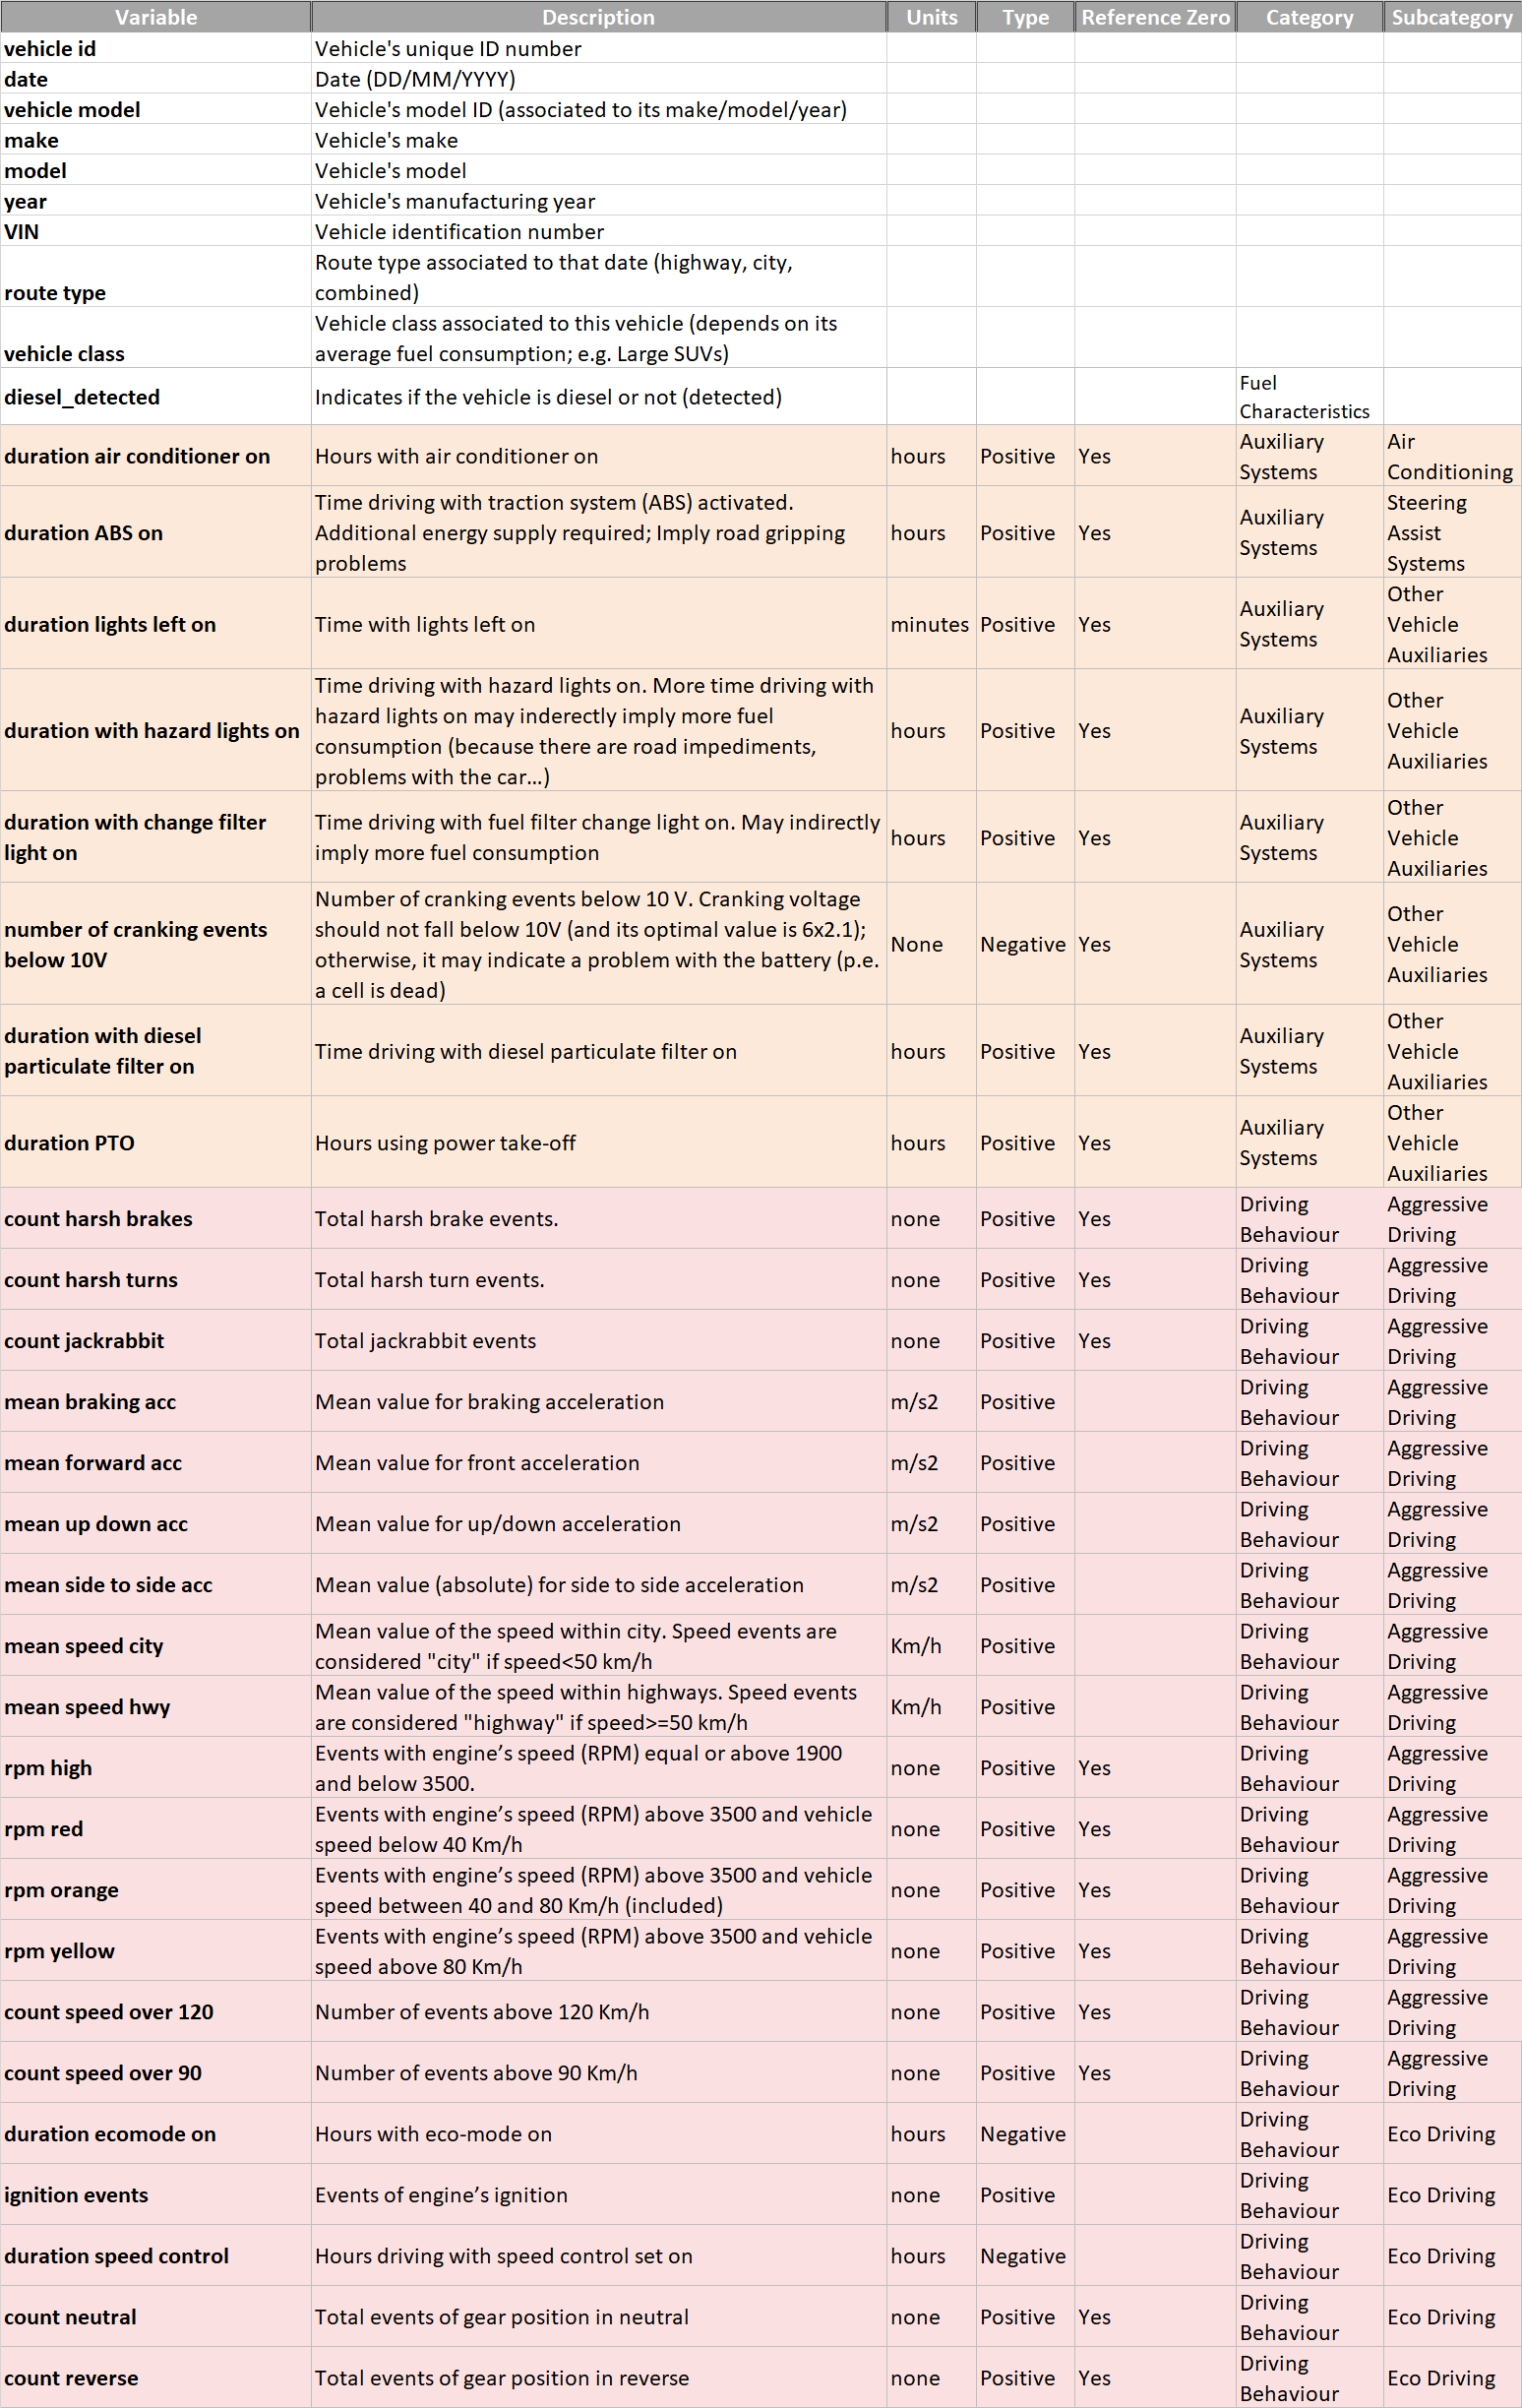
\includegraphics[width=395pt, height=580pt, keepaspectratio]{figures/chapter6_LucaFleet/FARUsedpt1.png}
  \end{tabular} 
  \caption{General variables and features used for predicting the fuel usage, with their associated categories and subcategories, according to \parencite{zacharof2016review} for Auxiliary Systems and Driving Behaviour \label{table:annex-FARUsedpt1}.}
\end{table}

\begin{table}[h!]
\centering
 \begin{tabular}{c@{\qquad}c@{\qquad}c}
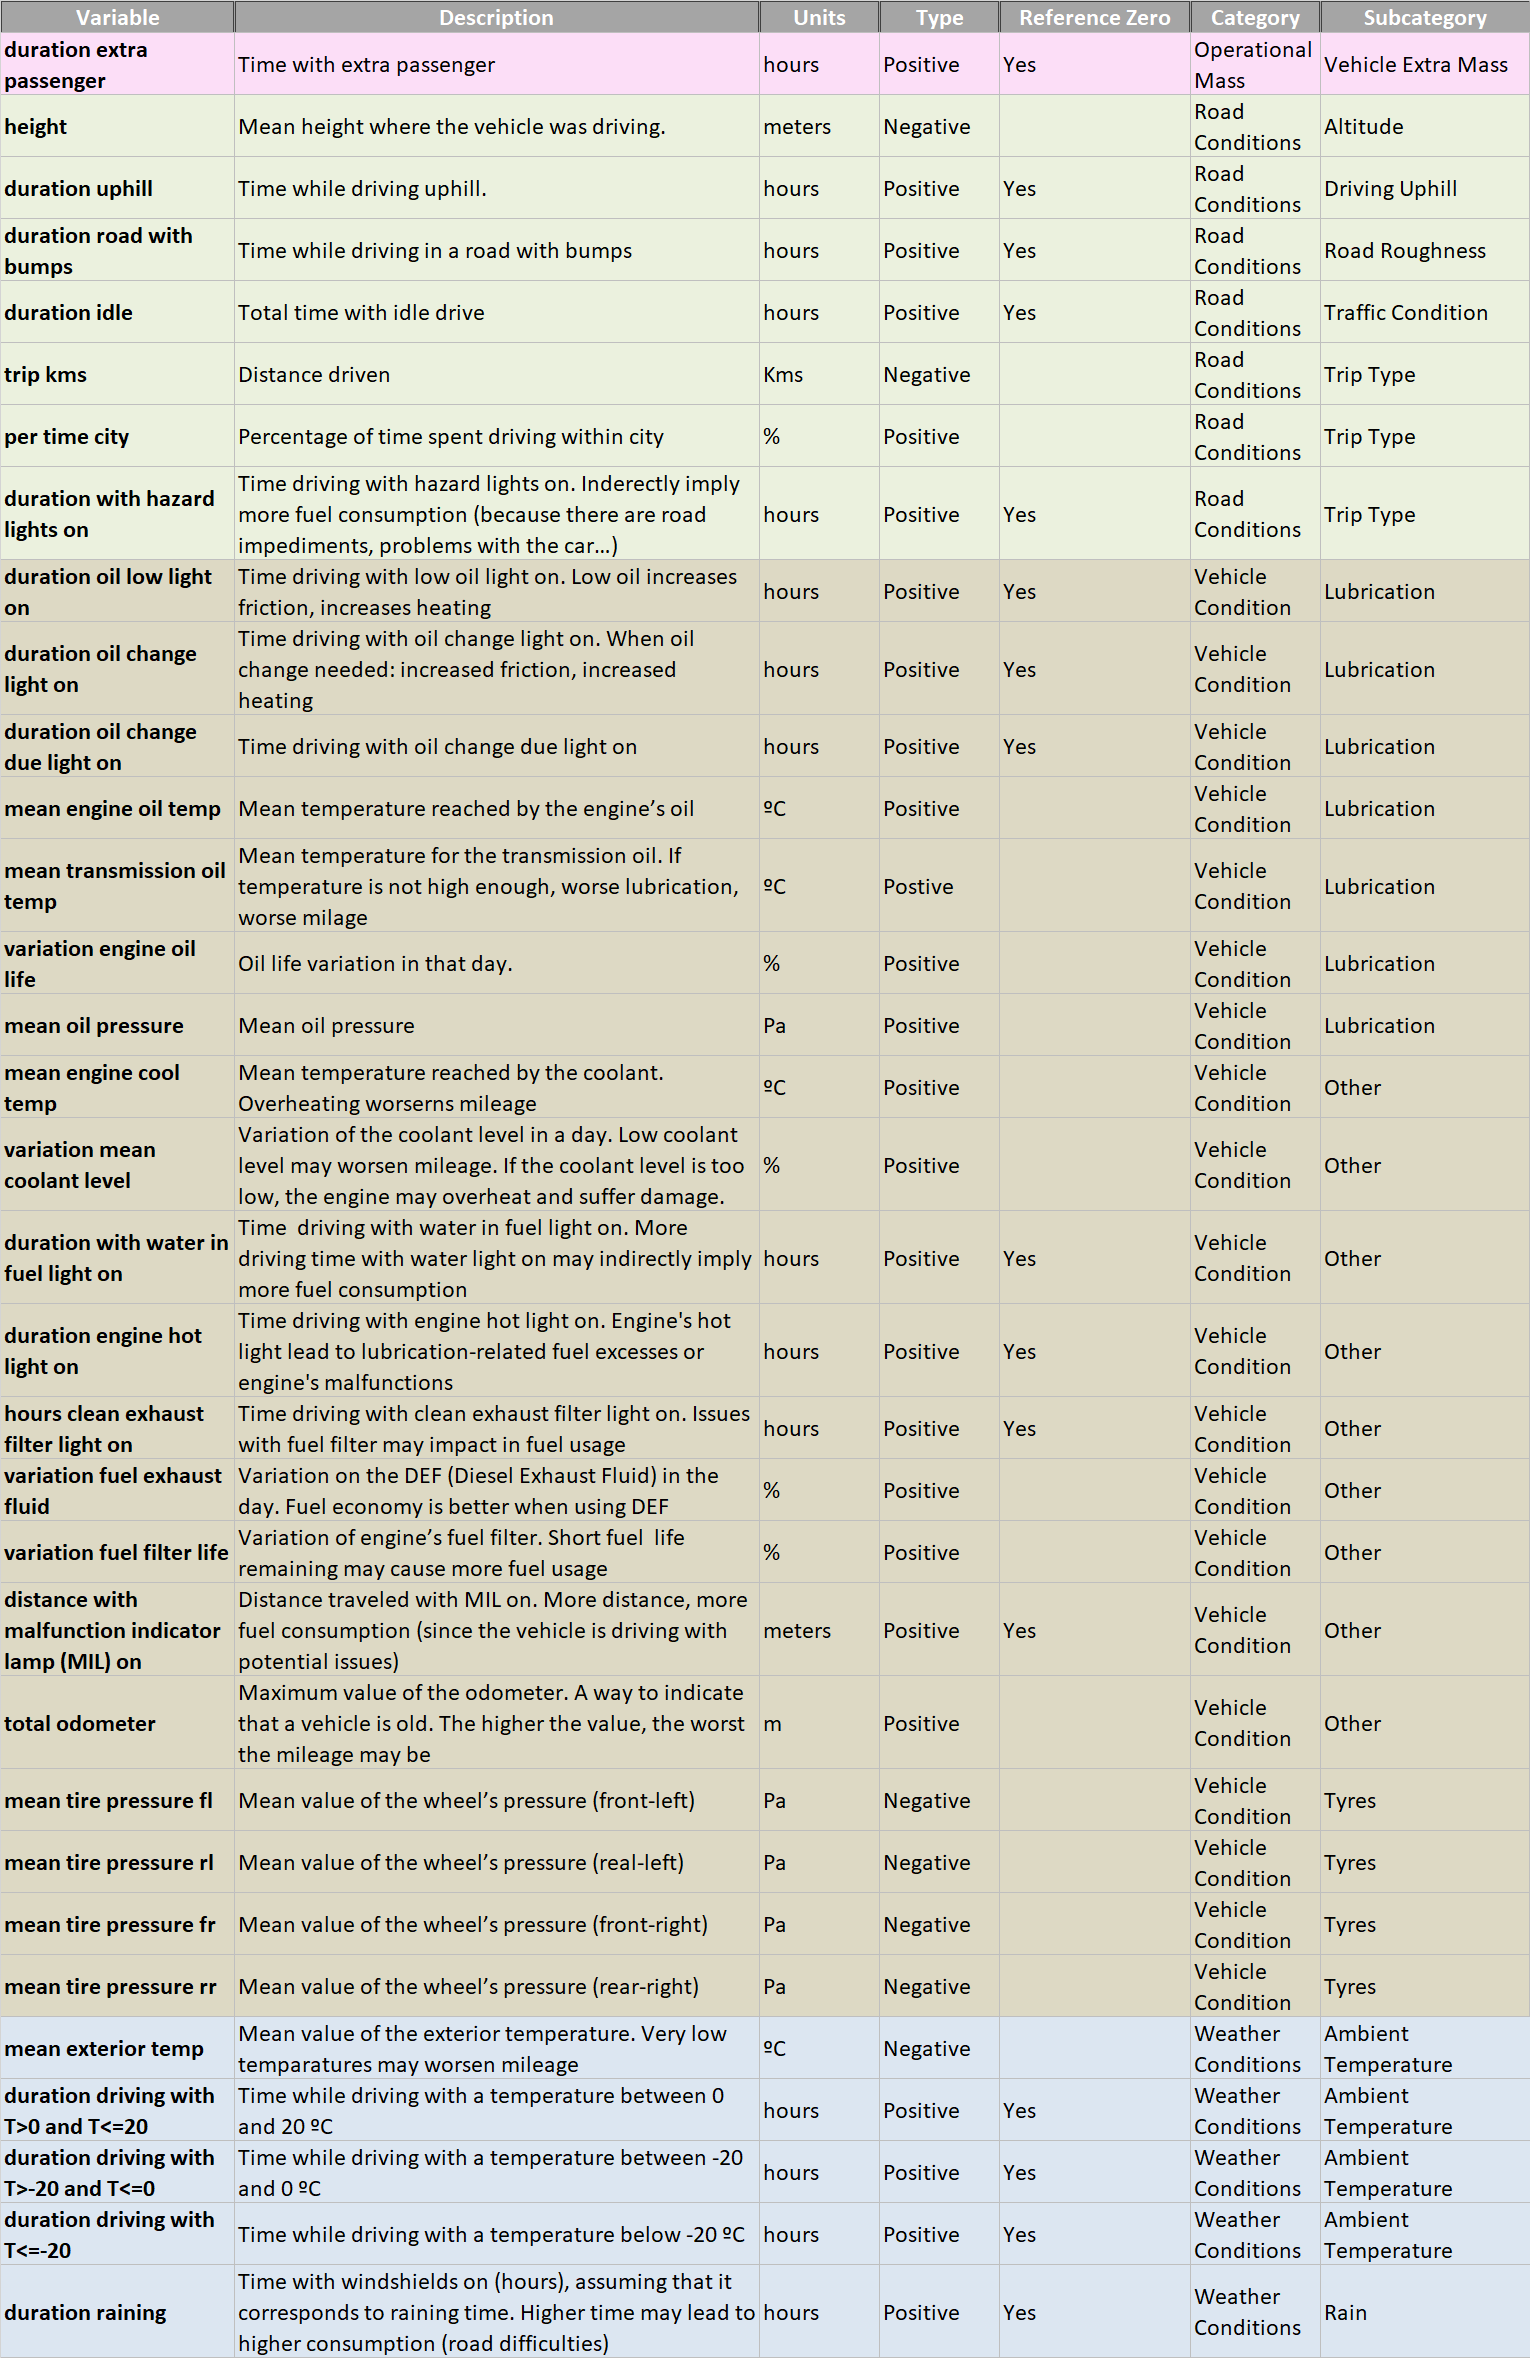
\includegraphics[width=395pt, height=580pt, keepaspectratio]{figures/chapter6_LucaFleet/FARUsedpt2.png}
  \end{tabular} 
  \caption{Features used for predicting the fuel usage, with their associated categories and subcategories, according to \parencite{zacharof2016review} for Operational Mass, Road Conditions, Vehicle Conditions and Weather Conditions  \label{table:annex-FARUsedpt2}}
\end{table}

Column "Name" includes a descriptive name for each of the features, and column "Description" contains a descriptive text about each of them. "Unit" indicates the metric units associated to each of the features, and "Notes" contains a description about some of the variables and why they may impact in fuel consumption (particularly for the ones that are not trivial). The column "Type" shows the type of impact that those features have in fuel consumption. If the type is "Positive" it indicates that increasing that feature value will normally \textit{increase} fuel usage. An example of this is the number of events with high RPM (Revolutions Per Minute); more events lead to more fuel consumption. On the contrary, if the type is "Negative", it indicates that increasing that feature value will normally \textit{decrease} fuel usage. An example of this is the time using speed control; more time using it should lower the fuel consumption (versus not using it). Another example is the tire pressure; when it decreases, the fuel used will increase. Column "Reference Zero" indicates the columns that in order to see the impact in the fuel consumption are set to zero. For instance, for obtaining the feature impact for a variable like "rpm\_high", this variable is set to 0 for calculating the reduction in the fuel consumption due to it by seeing the decrease with respect to the current feature value. For the remaining features, the reference is, by default, the median value for that feature over the vehicles with fuel inliers from the same vehicle model.
Finally, columns "Category" and "Subcategory" refer directly to the same columns from \hyperref[table:ch2-sota-factors-table]{Table} \ref{table:ch2-sota-factors-table} from \parencite{zacharof2016review}. The columns that do not have a value in both of these columns are columns that are not features used for explaining the fuel (they are relevant for the data set, and some of them are even used in the model, like the vehicle model, but they are not used for explanations). Among these columns is the main driving context detected for each day ("route\_type"). This is calculated as follows:


\newpage 

\ % The empty page

\newpage
\begin{itemize}
    \item IF $per\_time\_city \leq low\_th\_time$ AND $trip\_kms \geq th\_kms$ THEN $route\_type = hwy$
    \item ELSE IF $per\_time\_city \geq high\_th\_time$ AND $trip\_kms \leq th\_kms$ THEN $route\_type = city$
    \item ELSE $route\_type = combined$
\end{itemize}

With $th\_kms = 30$, $low\_th\_time = 0.5$ and $high\_th\_time = 0.65$.
Thus, we categorize each vehicle-date with a particular route type that may be "city", "highway" or "combined", depending on the total trip kms (trip\_kms) and the value of the variable per\_time\_city. An example of this route type categorization, using the threshold values aforementioned, appears in \hyperref[figure:annex-split-city-comb-hwy]{Figure} \ref{figure:annex-split-city-comb-hwy}.

\begin{figure}[h!]
\centering
 \begin{tabular}{c@{\qquad}c@{\qquad}c}
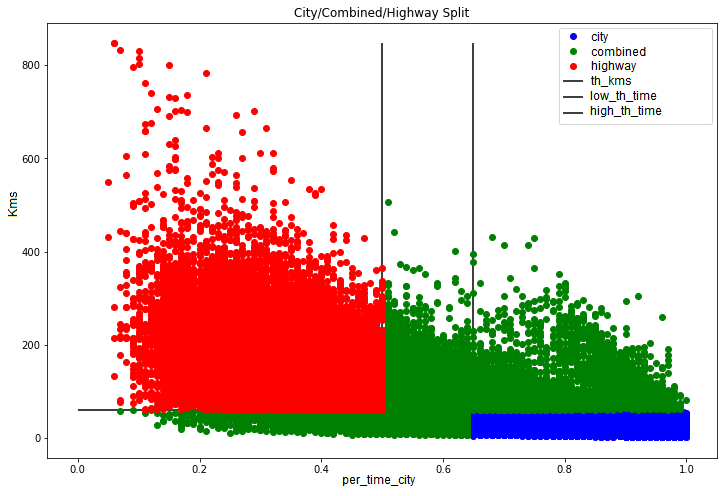
\includegraphics[width=0.6 \columnwidth]{figures/chapter6_LucaFleet/split_city_comb_hwy.png}
  \end{tabular} 
  \caption{Daily categorization of route types based on the trip distance (Km) and per\_time\_city for the data set D1 from \hyperref[subsec:ch6-DataFleet]{Subsection} \ref{subsec:ch6-DataFleet}.  \label{figure:annex-split-city-comb-hwy}}
\end{figure}

Also, the data sets contain different types of vehicles that are identified with two groups of variables. The first one is the vehicle's make, model, year and fuel type. Since fuel consumption depends on the type of vehicle (among other things), we use the Vehicle's Identification Number (VIN) to identify those variables.
Along with that, since some models may have similar fuel consumption, we add an additional variable, named vehicle class, that groups together those vehicles (e.g. "Large Pick-Ups"). This vehicle class is inferred directly from the historical mean fuel consumption, and is detailed in \hyperref[table:annex-vehicle-class]{Table} \ref{table:annex-vehicle-class}, where classify each vehicle from \hyperref[table:ch6-data-description]{Table} \ref{table:ch6-data-description} in one of the classes from \parencite[p.~18]{national2010technologies}.
With that, we are conducting the analyses over fleets of vehicles that are different among themselves, in order to provide results that are as general as possible. Following this, for the different fleets described in \hyperref[subsec:ch6-DataFleet]{Subsection} \ref{subsec:ch6-DataFleet}, we see passenger fleets of vehicles (such as D1), as well as heavy-duty vehicles, like trucks, (such as D3). 

\begin{table}[h!]
\resizebox{\textwidth}{!}{%
\begin{tabular}{@{}lllllll@{}}
\toprule
\textbf{Class} & \textbf{Applications}                                                                                                                                & \textbf{Gross Weight Range (lb)} & \textbf{L100Km\_min} & \textbf{L100Km\_max} & \textbf{L100Km\_med} & \textbf{Vehicle Class} \\ \midrule
1c             & Cars only                                                                                                                                            & 3,200 to 6,000                        & 7.12                 & 9.41                 & 8.27                 & 0                      \\
1t             & \begin{tabular}[c]{@{}l@{}}Minivans, Small SUVs, \\ Small Pick-Ups\end{tabular}                                                                      & 4,000 to 6,000                        & 9.40                 & 11.76                & 10.58                & 1                      \\
2a             & Large SUVs, Standard Pick-Ups                                                                                                                        & 6,001 to 8,500                        & 11.20                & 11.76                & 11.48                & 2                      \\
2b             & \begin{tabular}[c]{@{}l@{}}Large Pick-Up, Utility Van,\\  Multi-Purpose, Mini-Bus, Step Van\end{tabular}                                             & 8,501 to 10,000                      & 15.68                & 23.52                & 19.60                & 3                      \\
3              & \begin{tabular}[c]{@{}l@{}}Utility Van, Multi-Purpose,\\  Mini-Bus, Step Van\end{tabular}                                                            & 10,001 to 14,000                    & 18.09                & 29.40                & 23.74                & 4                      \\
4              & \begin{tabular}[c]{@{}l@{}}City Delivery, Parcel Delivery, \\ Large Walk-in, Bucket, Landscaping\end{tabular}                                        & 14,001 to 16,000                    & 19.60                & 33.60                & 26.60                & 5                      \\
5              & \begin{tabular}[c]{@{}l@{}}City Delivery, Parcel Delivery,\\  Large Walk-in, Bucket\end{tabular}                                                     & 16,001 to 19,500                    & 19.60                & 39.20                & 29.40                & 6                      \\
6              & \begin{tabular}[c]{@{}l@{}}City Delivery, School Bus, \\ Large Walk-in, Bucket\end{tabular}                                                          & 19,501 to 26,000                    & 19.60                & 47.04                & 33.32                & 7                      \\
7              & \begin{tabular}[c]{@{}l@{}}City Bus, Furniture, Refrigerated, \\ Refuse, Fuel Tanker Dump,Tow, \\ Concrete, Fire Engine, Tractor-Trailer\end{tabular} & 26,001 to 33,000                    & 29.40                & 58.80                & 44.10                & 8                      \\
8b             & \begin{tabular}[c]{@{}l@{}}Tractor-Trailer: Van, Refrigerated, \\ Bulk Tanker, Flat Bed (combination trucks)\end{tabular}                            & 33,001 to 80,000                    & 31.36                & 58.80                & 45.08                & 9                      \\
8a             & \begin{tabular}[c]{@{}l@{}}Dump, Refuse, Concrete, Furniture,\\  City Bus, Tow, Fire Engine \\ (straight trucks)\end{tabular}                        & 33,001 to 80,000                    & 39.20                & 94.09                & 66.64                & 10                     \\ \bottomrule
\end{tabular}%
}
\caption{Vehicle classes according to their average fuel consumption, as appears in \parencite[p.~18]{national2010technologies} }
\label{table:annex-vehicle-class}
\end{table}

Considering the data sets described in \hyperref[subsec:ch6-DataFleet]{Subsection} \ref{subsec:ch6-DataFleet}, the amount of vehicles per vehicle class from \hyperref[table:annex-vehicle-class]{Table} \ref{table:annex-vehicle-class} appears in \hyperref[table:annex-data-description]{Table} \ref{table:annex-data-description}.

\begin{table}[h!]
\centering
\resizebox{0.9\textwidth}{!}{%
\begin{tabular}{@{}lllllllllllllllll@{}}
\toprule
\textbf{Fleet} &
  \textbf{Class 0} &
  \textbf{Class 1} &
  \textbf{Class 2} &
  \textbf{Class 3} &
  \textbf{Class 4} &
  \textbf{Class 5} &
  \textbf{Class 6} &
  \textbf{Class 7} &
  \textbf{Class 8} &
  \textbf{Class 9}  &
  \textbf{Class 10} \\ \midrule
D1 & 1479 & 35  & 1   & 37  & 0  & 0 & 0  & 0 & 0  & 0  & 0  \\
D2 & 205  & 697 & 75  & 588 & 0  & 3 & 0  & 0 & 0  & 0  & 0  \\
D3 & 243  & 5   & 1   & 9   & 10 & 5 & 13 & 9 & 21 & 0  & 0  \\
D4 & 4    & 178 & 61  & 9   & 0  & 0 & 0  & 0 & 0  & 0  & 0  \\
D5 & 165  & 0   & 0   & 0   & 0  & 0 & 0  & 0 & 0  & 0  & 0  \\
D6 & 1    & 28  & 100 & 5   & 3  & 0 & 0  & 0 & 5  & 1  & 0  \\
D7 & 0    & 0   & 0   & 2   & 3  & 0 & 0  & 0 & 10 & 18 & 0  \\
D8 & 5    & 15  & 0   & 0   & 0  & 0 & 0  & 0 & 0  & 0  & 0  \\
D9 & 1    & 0   & 0   & 0   & 0  & 0 & 0  & 0 & 2  & 0  & 0  \\ \bottomrule
\end{tabular}%
}
\caption{Data set description for the number and type of vehicles.}
\label{table:annex-data-description}
\end{table}


\newpage
\subsection{Results for the analyses of model performance for vehicle fuel consumption}\label{subsec:ch6-annex-fleet-results-performance-contrast}
\begin{table}[h!]
\centering
\resizebox{380pt}{!}{%
\begin{tabular}{llllllllllll}
\textbf{model\_1} &
  \textbf{model\_2} &
  \textbf{metric} &
  \textbf{D1\_m1} &
  \textbf{D1\_m2} &
  \textbf{p1} &
  \textbf{D3\_m1} &
  \textbf{D3\_m2} &
  \textbf{p2} &
  \textbf{D7\_m1} &
  \textbf{D7\_m2} &
  \textbf{p3} \\ \hline
EBM           & xgboost        & explained\_variance\_score & 0.67  & 0.72  & 0.0  & 0.56  & 0.62  & 0.0  & 0.63  & 0.66  & 0.98 \\
EBM           & xgboost        & max\_error                 & 27.8  & 24.84 & 0.0  & 27.22 & 27.0  & 0.21 & 21.12 & 19.96 & 0.99 \\
EBM           & xgboost        & mean\_absolute\_error      & 0.65  & 0.62  & 0.0  & 1.21  & 1.12  & 0.0  & 6.26  & 6.04  & 0.27 \\
EBM           & xgboost        & mean\_squared\_error       & 1.25  & 1.14  & 0.0  & 2.28  & 2.16  & 0.0  & 8.42  & 8.2   & 0.99 \\
EBM           & xgboost        & median\_absolute\_error    & 0.42  & 0.41  & 0.0  & 0.67  & 0.63  & 0.0  & 4.66  & 4.5   & 0.09 \\
EBM           & xgboost        & r2\_score                  & 0.67  & 0.72  & 0.0  & 0.56  & 0.62  & 0.0  & 0.59  & 0.65  & 0.83 \\
EBM           & lightgbm       & explained\_variance\_score & 0.67  & 0.69  & 0.0  & 0.56  & 0.6   & 0.0  & 0.63  & 0.68  & 0.05 \\
EBM           & lightgbm       & max\_error                 & 27.8  & 26.49 & 0.0  & 27.22 & 26.72 & 0.3  & 21.12 & 19.44 & 0.48 \\
EBM           & lightgbm       & mean\_absolute\_error      & 0.65  & 0.64  & 0.0  & 1.21  & 1.16  & 0.0  & 6.26  & 5.68  & 0.0  \\
EBM           & lightgbm       & mean\_squared\_error       & 1.25  & 1.2   & 0.0  & 2.28  & 2.18  & 0.0  & 8.42  & 7.64  & 0.04 \\
EBM           & lightgbm       & median\_absolute\_error    & 0.42  & 0.42  & 0.24 & 0.67  & 0.66  & 0.76 & 4.66  & 4.23  & 0.07 \\
EBM           & lightgbm       & r2\_score                  & 0.67  & 0.69  & 0.0  & 0.56  & 0.6   & 0.0  & 0.59  & 0.68  & 0.08 \\
EBM           & linear\_model  & explained\_variance\_score & 0.67  & 0.2   & 0.0  & 0.56  & 0.19  & 0.0  & 0.63  & 0.29  & 0.0  \\
EBM           & linear\_model  & max\_error                 & 27.8  & 28.05 & 0.0  & 27.22 & 32.08 & 0.0  & 21.12 & 21.82 & 0.25 \\
EBM           & linear\_model  & mean\_absolute\_error      & 0.65  & 1.26  & 0.0  & 1.21  & 1.75  & 0.0  & 6.26  & 9.72  & 0.0  \\
EBM           & linear\_model  & mean\_squared\_error       & 1.25  & 1.9   & 0.0  & 2.28  & 3.14  & 0.0  & 8.42  & 11.47 & 0.0  \\
EBM           & linear\_model  & median\_absolute\_error    & 0.42  & 0.91  & 0.0  & 0.67  & 1.04  & 0.0  & 4.66  & 9.25  & 0.0  \\
EBM           & linear\_model  & r2\_score                  & 0.67  & 0.2   & 0.0  & 0.56  & 0.19  & 0.0  & 0.59  & 0.28  & 0.0  \\
EBM           & EBM\_var & explained\_variance\_score & 0.67  & 0.7   & 0.02 & 0.56  & 0.6   & 0.05 & 0.63  & 0.62  & 0.77 \\
EBM           & EBM\_var & max\_error                 & 27.8  & 27.48 & 0.75 & 27.22 & 29.7  & 0.39 & 21.12 & 21.57 & 0.63 \\
EBM           & EBM\_var & mean\_absolute\_error      & 0.65  & 0.62  & 0.0  & 1.21  & 1.13  & 0.0  & 6.26  & 5.76  & 0.44 \\
EBM           & EBM\_var & mean\_squared\_error       & 1.25  & 1.14  & 0.07 & 2.28  & 2.29  & 0.55 & 8.42  & 8.04  & 0.85 \\
EBM           & EBM\_var & median\_absolute\_error    & 0.42  & 0.4   & 0.0  & 0.67  & 0.6   & 0.0  & 4.66  & 4.46  & 0.54 \\
EBM           & EBM\_var & r2\_score                  & 0.67  & 0.7   & 0.03 & 0.56  & 0.6   & 0.05 & 0.59  & 0.62  & 0.83 \\
xgboost       & lightgbm       & explained\_variance\_score & 0.72  & 0.69  & 0.0  & 0.62  & 0.6   & 0.01 & 0.66  & 0.68  & 0.06 \\
xgboost       & lightgbm       & max\_error                 & 24.84 & 26.49 & 0.0  & 27.0  & 26.72 & 0.69 & 19.96 & 19.44 & 0.53 \\
xgboost       & lightgbm       & mean\_absolute\_error      & 0.62  & 0.64  & 0.0  & 1.12  & 1.16  & 0.0  & 6.04  & 5.68  & 0.29 \\
xgboost       & lightgbm       & mean\_squared\_error       & 1.14  & 1.2   & 0.0  & 2.16  & 2.18  & 0.01 & 8.2   & 7.64  & 0.05 \\
xgboost       & lightgbm       & median\_absolute\_error    & 0.41  & 0.42  & 0.0  & 0.63  & 0.66  & 0.0  & 4.5   & 4.23  & 0.64 \\
xgboost       & lightgbm       & r2\_score                  & 0.72  & 0.69  & 0.0  & 0.62  & 0.6   & 0.01 & 0.65  & 0.68  & 0.04 \\
xgboost       & linear\_model  & explained\_variance\_score & 0.72  & 0.2   & 0.0  & 0.62  & 0.19  & 0.0  & 0.66  & 0.29  & 0.0  \\
xgboost       & linear\_model  & max\_error                 & 24.84 & 28.05 & 0.0  & 27.0  & 32.08 & 0.0  & 19.96 & 21.82 & 0.3  \\
xgboost       & linear\_model  & mean\_absolute\_error      & 0.62  & 1.26  & 0.0  & 1.12  & 1.75  & 0.0  & 6.04  & 9.72  & 0.0  \\
xgboost       & linear\_model  & mean\_squared\_error       & 1.14  & 1.9   & 0.0  & 2.16  & 3.14  & 0.0  & 8.2   & 11.47 & 0.0  \\
xgboost       & linear\_model  & median\_absolute\_error    & 0.41  & 0.91  & 0.0  & 0.63  & 1.04  & 0.0  & 4.5   & 9.25  & 0.0  \\
xgboost       & linear\_model  & r2\_score                  & 0.72  & 0.2   & 0.0  & 0.62  & 0.19  & 0.0  & 0.65  & 0.28  & 0.0  \\
xgboost       & EBM\_var & explained\_variance\_score & 0.72  & 0.7   & 0.11 & 0.62  & 0.6   & 0.1  & 0.66  & 0.62  & 0.9  \\
xgboost       & EBM\_var & max\_error                 & 24.84 & 27.48 & 0.64 & 27.0  & 29.7  & 0.3  & 19.96 & 21.57 & 0.85 \\
xgboost       & EBM\_var & mean\_absolute\_error      & 0.62  & 0.62  & 0.42 & 1.12  & 1.13  & 0.34 & 6.04  & 5.76  & 0.89 \\
xgboost       & EBM\_var & mean\_squared\_error       & 1.14  & 1.14  & 0.17 & 2.16  & 2.29  & 0.12 & 8.2   & 8.04  & 0.85 \\
xgboost       & EBM\_var & median\_absolute\_error    & 0.41  & 0.4   & 0.02 & 0.63  & 0.6   & 0.0  & 4.5   & 4.46  & 0.6  \\
xgboost       & EBM\_var & r2\_score                  & 0.72  & 0.7   & 0.1  & 0.62  & 0.6   & 0.1  & 0.65  & 0.62  & 0.96 \\
lightgbm      & linear\_model  & explained\_variance\_score & 0.69  & 0.2   & 0.0  & 0.6   & 0.19  & 0.0  & 0.68  & 0.29  & 0.0  \\
lightgbm      & linear\_model  & max\_error                 & 26.49 & 28.05 & 0.0  & 26.72 & 32.08 & 0.0  & 19.44 & 21.82 & 0.01 \\
lightgbm      & linear\_model  & mean\_absolute\_error      & 0.64  & 1.26  & 0.0  & 1.16  & 1.75  & 0.0  & 5.68  & 9.72  & 0.0  \\
lightgbm      & linear\_model  & mean\_squared\_error       & 1.2   & 1.9   & 0.0  & 2.18  & 3.14  & 0.0  & 7.64  & 11.47 & 0.0  \\
lightgbm      & linear\_model  & median\_absolute\_error    & 0.42  & 0.91  & 0.0  & 0.66  & 1.04  & 0.0  & 4.23  & 9.25  & 0.0  \\
lightgbm      & linear\_model  & r2\_score                  & 0.69  & 0.2   & 0.0  & 0.6   & 0.19  & 0.0  & 0.68  & 0.28  & 0.0  \\
lightgbm      & EBM\_var & explained\_variance\_score & 0.69  & 0.7   & 0.91 & 0.6   & 0.6   & 0.28 & 0.68  & 0.62  & 0.62 \\
lightgbm      & EBM\_var & max\_error                 & 26.49 & 27.48 & 0.91 & 26.72 & 29.7  & 0.38 & 19.44 & 21.57 & 0.43 \\
lightgbm      & EBM\_var & mean\_absolute\_error      & 0.64  & 0.62  & 0.0  & 1.16  & 1.13  & 0.53 & 5.68  & 5.76  & 0.6  \\
lightgbm      & EBM\_var & mean\_squared\_error       & 1.2   & 1.14  & 0.97 & 2.18  & 2.29  & 0.21 & 7.64  & 8.04  & 0.37 \\
lightgbm      & EBM\_var & median\_absolute\_error    & 0.42  & 0.4   & 0.0  & 0.66  & 0.6   & 0.0  & 4.23  & 4.46  & 0.73 \\
lightgbm      & EBM\_var & r2\_score                  & 0.69  & 0.7   & 0.84 & 0.6   & 0.6   & 0.29 & 0.68  & 0.62  & 0.55 \\
linear\_model & EBM\_var & explained\_variance\_score & 0.2   & 0.7   & 0.0  & 0.19  & 0.6   & 0.0  & 0.29  & 0.62  & 0.0  \\
linear\_model & EBM\_var & max\_error                 & 28.05 & 27.48 & 0.43 & 32.08 & 29.7  & 0.08 & 21.82 & 21.57 & 0.61 \\
linear\_model & EBM\_var & mean\_absolute\_error      & 1.26  & 0.62  & 0.0  & 1.75  & 1.13  & 0.0  & 9.72  & 5.76  & 0.0  \\
linear\_model & EBM\_var & mean\_squared\_error       & 1.9   & 1.14  & 0.0  & 3.14  & 2.29  & 0.0  & 11.47 & 8.04  & 0.0  \\
linear\_model & EBM\_var & median\_absolute\_error    & 0.91  & 0.4   & 0.0  & 1.04  & 0.6   & 0.0  & 9.25  & 4.46  & 0.0  \\
linear\_model & EBM\_var & r2\_score                  & 0.2   & 0.7   & 0.0  & 0.19  & 0.6   & 0.0  & 0.28  & 0.62  & 0.0 
\end{tabular}
}
\caption{Model metrics results for model comparison. Columns with "D" indicate the median value for that combination (for instance, D3\_m2 is the median value for model\_2 with the metric considered at data set 3). P indicates the p-value for that data set.}
\label{table:annex-model-metrics-contrast}
\end{table}


\newpage
\subsection{Results for the analyses of XAI for vehicle fuel consumption}\label{subsec:annex-fleet-results}
\begin{table*}[]
\centering
\resizebox{305pt}{!}{%
\begin{tabular}{@{}llllllll@{}}
\toprule
\textbf{Data set} & \textbf{Method 1} & \textbf{Method 2} & \textbf{Metric}   & \textbf{Taxonomy}  & \textbf{Mean 1} & \textbf{Mean 2} & \textbf{p-value} \\ \midrule
Large  & EBM\_var & EBM     & n\_features\_used & Representativeness & \textbf{4.047} & 3.872          & 0.0   \\
Large  & monoGAM        & EBM     & n\_features\_used & Representativeness & 3.888          & \textbf{4.008} & 0.0   \\
Large             & EBM\_var    & monoGAM           & n\_features\_used & Representativeness & \textbf{4.166}  & 3.871           & 0.0              \\
Medium & EBM\_var & EBM     & n\_features\_used & Representativeness & \textbf{5.187} & 4.752          & 0.0   \\
Medium & monoGAM        & EBM     & n\_features\_used & Representativeness & 4.352          & \textbf{4.811} & 0.0   \\
Medium            & EBM\_var    & monoGAM           & n\_features\_used & Representativeness & \textbf{5.215}  & 4.324           & 0.0              \\
Small  & EBM\_var & EBM     & n\_features\_used & Representativeness & 2.808          & 2.803          & 0.408 \\
Small  & monoGAM        & EBM     & n\_features\_used & Representativeness & \textbf{4.32}  & 2.958          & 0.0   \\
Small  & EBM\_var & monoGAM & n\_features\_used & Representativeness & 3.15           & \textbf{4.332} & 0.0   \\
Large  & EBM\_var & EBM     & rel\_importance   & Representativeness & 0.139          & \textbf{0.175} & 0.0   \\
Large  & monoGAM        & EBM     & rel\_importance   & Representativeness & 0.099          & \textbf{0.181} & 0.0   \\
Large  & EBM\_var & monoGAM & rel\_importance   & Representativeness & \textbf{0.143} & 0.099          & 0.0   \\
Medium & EBM\_var & EBM     & rel\_importance   & Representativeness & 0.13           & \textbf{0.177} & 0.0   \\
Medium & monoGAM        & EBM     & rel\_importance   & Representativeness & 0.126          & \textbf{0.179} & 0.0   \\
Medium & EBM\_var & monoGAM & rel\_importance   & Representativeness & \textbf{0.131} & 0.125          & 0.0   \\
Small  & EBM\_var & EBM     & rel\_importance   & Representativeness & 0.066          & \textbf{0.184} & 0.0   \\
Small  & monoGAM        & EBM     & rel\_importance   & Representativeness & \textbf{0.22}  & 0.103          & 0.0   \\
Small  & EBM\_var & monoGAM & rel\_importance   & Representativeness & 0.077          & \textbf{0.217} & 0.0   \\
Large  & EBM\_var & EBM     & xai\_mape         & Precision          & 0.261          & 0.267          & 0.406 \\
Large  & monoGAM        & EBM     & xai\_mape         & Precision          & 0.278          & \textbf{0.264} & 0.033 \\
Large  & EBM\_var & monoGAM & xai\_mape         & Precision          & 0.258 & 0.277          & 0.079 \\
Medium & EBM\_var & EBM     & xai\_mape         & Precision          & 0.275          & 0.287          & 0.358 \\
Medium & monoGAM        & EBM     & xai\_mape         & Precision          & 0.413          & \textbf{0.286} & 0.0   \\
Medium & EBM\_var & monoGAM & xai\_mape         & Precision          & \textbf{0.275} & 0.407          & 0.0   \\
Small  & EBM\_var & EBM     & xai\_mape         & Precision          & 0.499          & 0.51           & 0.7   \\
Small  & monoGAM        & EBM     & xai\_mape         & Precision          & 0.497          & 0.525          & 0.424 \\
Small  & EBM\_var & monoGAM & xai\_mape         & Precision          & 0.513          & 0.497          & 0.589 \\
Large  & EBM\_var & EBM     & stability\_error  & Stability          & 0.392          & 0.358          & 0.164 \\
Large  & monoGAM        & EBM     & stability\_error  & Stability          & 0.381          & 0.357          & 0.977 \\
Large  & EBM\_var & monoGAM & stability\_error  & Stability          & 0.396          & 0.381          & 0.351 \\
Medium & EBM\_var & EBM     & stability\_error  & Stability          & 0.826          & \textbf{0.661} & 0.0   \\
Medium & monoGAM        & EBM     & stability\_error  & Stability          & 0.943          & \textbf{0.664} & 0.0   \\
Medium & EBM\_var & monoGAM & stability\_error  & Stability          & \textbf{0.828} & 0.945          & 0.0   \\
Small  & EBM\_var & EBM     & stability\_error  & Stability          & \textbf{2.871} & 2.874          & 0.0   \\
Small  & monoGAM        & EBM     & stability\_error  & Stability          & \textbf{1.444} & 2.097          & 0.0   \\
Small  & EBM\_var & monoGAM & stability\_error  & Stability          & 2.025          & 1.438          & 0.075 \\
Large  & EBM\_var & EBM     & per\_var          & Contrastiveness    & \textbf{0.252} & 0.222          & 0.0   \\
Large  & monoGAM        & EBM     & per\_var          & Contrastiveness    & 0.162          & \textbf{0.23}  & 0.0   \\
Large  & EBM\_var & monoGAM & per\_var          & Contrastiveness    & \textbf{0.26}  & 0.161          & 0.0   \\
Medium & EBM\_var & EBM     & per\_var          & Contrastiveness    & \textbf{0.299} & 0.243          & 0.0   \\
Medium & monoGAM        & EBM     & per\_var          & Contrastiveness    & \textbf{0.266} & 0.245          & 0.007 \\
Medium & EBM\_var & monoGAM & per\_var          & Contrastiveness    & \textbf{0.299} & 0.263          & 0.0   \\
Small  & EBM\_var & EBM     & per\_var          & Contrastiveness    & 0.178          & \textbf{0.241} & 0.0   \\
Small  & monoGAM        & EBM     & per\_var          & Contrastiveness    & \textbf{0.32}  & 0.164          & 0.0   \\
Small  & EBM\_var & monoGAM & per\_var          & Contrastiveness    & 0.164          & \textbf{0.317} & 0.0   \\
Large  & EBM\_var & EBM     & per\_below        & Contrastiveness    & \textbf{0.796} & 0.768          & 0.001 \\
Large  & monoGAM        & EBM     & per\_below        & Contrastiveness    & 0.656          & \textbf{0.768} & 0.0   \\
Large  & EBM\_var & monoGAM & per\_below        & Contrastiveness    & \textbf{0.796} & 0.656          & 0.0   \\
Medium & EBM\_var & EBM     & per\_below        & Contrastiveness    & \textbf{0.712} & 0.67           & 0.0   \\
Medium & monoGAM        & EBM     & per\_below        & Contrastiveness    & 0.637          & \textbf{0.67}  & 0.0   \\
Medium & EBM\_var & monoGAM & per\_below        & Contrastiveness    & \textbf{0.712} & 0.637          & 0.0   \\
Small  & EBM\_var & EBM     & per\_below        & Contrastiveness    & \textbf{0.651} & 0.635          & 0.034 \\
Small  & monoGAM        & EBM     & per\_below        & Contrastiveness    & \textbf{0.818} & 0.635          & 0.0   \\
Small  & EBM\_var & monoGAM & per\_below        & Contrastiveness    & 0.651          & \textbf{0.818} & 0.0   \\
Large  & EBM\_var & EBM     & per\_mon          & Apriori Beliefs    & 0.544          & \textbf{0.602} & 0.0   \\
Large  & monoGAM        & EBM     & per\_mon          & Apriori Beliefs    & \textbf{1.0}   & 0.605          & 0.0   \\
Large  & EBM\_var & monoGAM & per\_mon          & Apriori Beliefs    & 0.543          & \textbf{1.0}   & 0.0   \\
Medium & EBM\_var & EBM     & per\_mon          & Apriori Beliefs    & 0.489          & \textbf{0.537} & 0.0   \\
Medium & monoGAM        & EBM     & per\_mon          & Apriori Beliefs    & \textbf{1.0}   & 0.54           & 0.0   \\
Medium & EBM\_var & monoGAM & per\_mon          & Apriori Beliefs    & 0.49           & \textbf{1.0}   & 0.0   \\
Small  & EBM\_var & EBM     & per\_mon          & Apriori Beliefs    & 0.549          & \textbf{0.571} & 0.005 \\
Small  & monoGAM        & EBM     & per\_mon          & Apriori Beliefs    & \textbf{1.0}   & 0.576          & 0.0   \\
Small  & EBM\_var & monoGAM & per\_mon          & Apriori Beliefs    & 0.549          & \textbf{1.0}   & 0.0   \\ \bottomrule

\end{tabular}%
}
\caption{Hypothesis contrast for XAI metrics regarding representativeness, precision, stability, contrastiveness, and apriori beliefs, comparing the results from EBM, EBM\_var, CGA2M+. Contrasts are carried out with statistically significant sample sizes, and using the same data set-vehicle-date (thus, the small differences in the mean value that the same algorithm can have for the same metric).}
\label{table:annex-xai-metrics-contrast}
\end{table*}

\newpage
\begin{table*}[]
\centering
\resizebox{320pt}{!}{%
\begin{tabular}{@{}llllllll@{}}
\toprule
\textbf{Data set} & \textbf{Method 1} & \textbf{Method 2} & \textbf{Metric} & \textbf{Taxonomy} & \textbf{Mean 1} & \textbf{Mean 2} & \textbf{p-value} \\ \midrule
Large  & EBM\_var & EBM     & n\_features\_used & Representativeness & 2.804          & \textbf{3.281} & 0.0   \\
Large  & monoGAM        & EBM     & n\_features\_used & Representativeness & \textbf{3.958} & 3.294          & 0.0   \\
Large  & EBM\_var & monoGAM & n\_features\_used & Representativeness & 2.825          & \textbf{3.977} & 0.0   \\
Medium & EBM\_var & EBM     & n\_features\_used & Representativeness & 2.563          & \textbf{2.616} & 0.083 \\
Medium & monoGAM        & EBM     & n\_features\_used & Representativeness & \textbf{4.447} & 2.586          & 0.0   \\
Medium & EBM\_var & monoGAM & n\_features\_used & Representativeness & 2.523          & \textbf{4.407} & 0.0   \\
Small  & EBM\_var & EBM     & n\_features\_used & Representativeness & 1.795          & \textbf{1.918} & 0.005 \\
Small  & monoGAM        & EBM     & n\_features\_used & Representativeness & \textbf{4.394} & 1.942          & 0.0   \\
Small  & EBM\_var & monoGAM & n\_features\_used & Representativeness & 1.905          & \textbf{4.45}  & 0.0   \\
Large  & EBM\_var & EBM     & rel\_importance   & Representativeness & 0.105          & \textbf{0.157} & 0.0   \\
Large  & monoGAM        & EBM     & rel\_importance   & Representativeness & 0.101          & \textbf{0.158} & 0.0   \\
Large  & EBM\_var & monoGAM & rel\_importance   & Representativeness & \textbf{0.106} & 0.101          & 0.0   \\
Medium & EBM\_var & EBM     & rel\_importance   & Representativeness & 0.076          & \textbf{0.108} & 0.0   \\
Medium & monoGAM        & EBM     & rel\_importance   & Representativeness & \textbf{0.128} & 0.106          & 0.0   \\
Medium & EBM\_var & monoGAM & rel\_importance   & Representativeness & 0.075          & \textbf{0.127} & 0.0   \\
Small  & EBM\_var & EBM     & rel\_importance   & Representativeness & 0.046          & \textbf{0.134} & 0.0   \\
Small  & monoGAM        & EBM     & rel\_importance   & Representativeness & \textbf{0.226} & 0.073          & 0.0   \\
Small  & EBM\_var & monoGAM & rel\_importance   & Representativeness & 0.055          & \textbf{0.217} & 0.0   \\
Large  & EBM\_var & EBM     & xai\_mape         & Precision          & 0.261          & 0.265          & 0.551 \\
Large  & monoGAM        & EBM     & xai\_mape         & Precision          & 0.279          & 0.262          & 0.162 \\
Large  & EBM\_var & monoGAM & xai\_mape         & Precision          & 0.259          & 0.28           & 0.232 \\
Medium & EBM\_var & EBM     & xai\_mape         & Precision          & 0.279          & 0.294          & 0.192 \\
Medium & monoGAM        & EBM     & xai\_mape         & Precision          & 0.415          & \textbf{0.294} & 0.0   \\
Medium & EBM\_var & monoGAM & xai\_mape         & Precision          & \textbf{0.279} & 0.408          & 0.0   \\
Small  & EBM\_var & EBM     & xai\_mape         & Precision          & 0.527          & 0.534          & 0.831 \\
Small  & monoGAM        & EBM     & xai\_mape         & Precision          & 0.509          & 0.534          & 0.27  \\
Small  & EBM\_var & monoGAM & xai\_mape         & Precision          & 0.517          & 0.496          & 0.292 \\
Large  & EBM\_var & EBM     & stability\_error  & Stability          & 0.36           & \textbf{0.319} & 0.017 \\
Large  & monoGAM        & EBM     & stability\_error  & Stability          & 0.381          & \textbf{0.311} & 0.0   \\
Large  & EBM\_var & monoGAM & stability\_error  & Stability          & \textbf{0.363} & 0.382          & 0.0   \\
Medium & EBM\_var & EBM     & stability\_error  & Stability          & 0.513          & \textbf{0.46}  & 0.0   \\
Medium & monoGAM        & EBM     & stability\_error  & Stability          & 0.953          & \textbf{0.461} & 0.0   \\
Medium & EBM\_var & monoGAM & stability\_error  & Stability          & \textbf{0.514} & 0.948          & 0.0   \\
Small  & EBM\_var & EBM     & stability\_error  & Stability          & 1.269          & 1.607          & 0.304 \\
Small  & monoGAM        & EBM     & stability\_error  & Stability          & 1.399          & \textbf{1.298} & 0.0   \\
Small  & EBM\_var & monoGAM & stability\_error  & Stability          & \textbf{0.787} & 1.337          & 0.0   \\
Large  & EBM\_var & EBM     & per\_var          & Contrastiveness    & 0.195          & \textbf{0.205} & 0.0   \\
Large  & monoGAM        & EBM     & per\_var          & Contrastiveness    & 0.165          & \textbf{0.206} & 0.0   \\
Large  & EBM\_var & monoGAM & per\_var          & Contrastiveness    & \textbf{0.196} & 0.166          & 0.0   \\
Medium & EBM\_var & EBM     & per\_var          & Contrastiveness    & \textbf{0.168} & 0.145          & 0.0   \\
Medium & monoGAM        & EBM     & per\_var          & Contrastiveness    & \textbf{0.273} & 0.142          & 0.0   \\
Medium & EBM\_var & monoGAM & per\_var          & Contrastiveness    & 0.165          & \textbf{0.269} & 0.0   \\
Small  & EBM\_var & EBM     & per\_var          & Contrastiveness    & 0.118          & \textbf{0.158} & 0.002 \\
Small  & monoGAM        & EBM     & per\_var          & Contrastiveness    & \textbf{0.323} & 0.105          & 0.0   \\
Small  & EBM\_var & monoGAM & per\_var          & Contrastiveness    & 0.099          & \textbf{0.317} & 0.0   \\
Large  & EBM\_var & EBM     & per\_below        & Contrastiveness    & 0.767          & 0.764          & 0.928 \\
Large  & monoGAM        & EBM     & per\_below        & Contrastiveness    & 0.656          & \textbf{0.764} & 0.0   \\
Large  & EBM\_var & monoGAM & per\_below        & Contrastiveness    & \textbf{0.767} & 0.656          & 0.0   \\
Medium & EBM\_var & EBM     & per\_below        & Contrastiveness    & \textbf{0.636} & 0.598          & 0.0   \\
Medium & monoGAM        & EBM     & per\_below        & Contrastiveness    & \textbf{0.637} & 0.598          & 0.0   \\
Medium & EBM\_var & monoGAM & per\_below        & Contrastiveness    & 0.636          & 0.637          & 0.771 \\
Small  & EBM\_var & EBM     & per\_below        & Contrastiveness    & 0.525          & 0.462          & 0.119 \\
Small  & monoGAM        & EBM     & per\_below        & Contrastiveness    & \textbf{0.818} & 0.462          & 0.0   \\
Small  & EBM\_var & monoGAM & per\_below        & Contrastiveness    & 0.525          & \textbf{0.818} & 0.0   \\ \bottomrule
\end{tabular}%
}
\caption{Hypothesis contrast for XAI metrics regarding representativeness, precision, stability, contrastiveness, and apriori beliefs, comparing the results from EBM, EBM\_var, CGA2M+, using the monotonicity filter in EBM and EBM\_var. Contrasts are carried out with statistically significant sample sizes, and using the same data set-vehicle-date (thus, the small differences in the mean value that the same algorithm can have for the same metric). }
\label{table:annex-xai-metrics-contrast-mono}
\end{table*}




